\chapter{Agent Skills and reusable engineering capabilities}

\section{Engineering principles}

The portable Agent Skills format packages task instructions in SKILL.md with metadata and optional supporting scripts, references and assets. Progressive disclosure allows a host to discover capabilities before reading complete instructions. Host-specific metadata and discovery paths are separate from the portable core. A skill is executable supply-chain material if it includes scripts or invokes tools; descriptive metadata cannot certify safety.\src{S1,O3,A3}

\section{Implementation approach}

Author one purpose per skill, use a name matching its directory and a description that states trigger conditions. Specify inputs, boundaries, workflow, evidence and stopping conditions. Store canonical packages in examples/skills and copy reviewed packages into the platform project skill directories. Evaluate positive triggers, unrelated prompts, malicious fixtures and output completeness. Review scripts and lock dependencies before installation.

\section{Verification and limitations}

The package includes seven original skills. Each is a task method rather than an authorization mechanism. Validate metadata and compare copied versions by checksum; require owner review for changes to scripts or external references.

Figure~\ref{fig:d8} illustrates the conceptual flow from Skill metadata to Execute under policy. The edges describe the proposed integration or control relationship, not undocumented internal calls.

\begin{figure}[htbp]\centering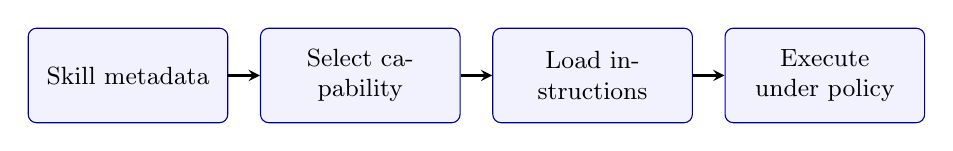
\begin{tikzpicture}[nodebox/.style={draw=blue!60!black,fill=blue!5,rounded corners=3pt,minimum height=12mm,text width=23mm,align=center,font=\small},>=stealth]
\node[nodebox] (n0) at (0.00,0.00) {Skill metadata};
\node[nodebox] (n1) at (2.95,0.00) {Select capability};
\node[nodebox] (n2) at (5.90,0.00) {Load instructions};
\node[nodebox] (n3) at (8.85,0.00) {Execute under policy};
\draw[->,thick] (n0.east) -- (n1.west);
\draw[->,thick] (n1.east) -- (n2.west);
\draw[->,thick] (n2.east) -- (n3.west);
\end{tikzpicture}
\caption{Agent Skill discovery (conceptual view).}\label{fig:d8}\end{figure}

\section{Chapter conclusion}

Apply the stated verification criteria before expanding the scope of this workflow. Record deviations, evidence and unresolved risks in the task record.
